% Final report for Real-time Fire & Smoke Detection with Alerts
% Engine: LuaLaTeX
\documentclass[12pt,a4paper]{article}

% Fonts and layout (LuaLaTeX)
\usepackage{fontspec}
\setmainfont{TeX Gyre Termes}
\usepackage[margin=1in]{geometry}
\usepackage{setspace}
\usepackage{microtype}
\usepackage{graphicx}
\usepackage{hyperref}
\usepackage{booktabs}
\usepackage{tabularx}
\usepackage{array}
\usepackage{enumitem}
\usepackage{titlesec}
\usepackage{caption}
\usepackage{tikz}
\usetikzlibrary{arrows.meta,positioning,shapes.geometric,fit,calc}

\hypersetup{colorlinks=true,linkcolor=black,urlcolor=blue,citecolor=black}
\setlist{nosep}
\onehalfspacing
\parindent=0pt
\parskip=6pt

% simple helper for optional images
\newcommand{\optionalinclude}[2]{% #1 file name, #2 width
  \IfFileExists{#1}{\includegraphics[width=#2]{#1}}{\fbox{\rule{0pt}{0.35#2}\rule{#2}{0pt}}}}

\begin{document}

% ---------------- Title Page ----------------
\begin{titlepage}
  \centering
  \begingroup\setstretch{1.05}
  {\itshape A\\[0.5em]}
  {\large Report Submitted\\[0.5em]}
  {\itshape for\\[0.5em]}
  {\LARGE\bfseries Project Review 1\\[0.5em]}
  {\itshape on the project entitled\\[0.5em]}
  {\LARGE\bfseries Real-time Fire \& Smoke Detection with Alerts\\[0.8em]}
  {\itshape in partial fulfilment for the course\\[0.4em]}
  {\Large BCSE407L - Computer Vision\\[0.4em]}
  {\small (Theory Only)\\[0.4em]}
  {\small Class ID: VL2025260102035\\[0.2em]}
  {\small Slot: D2+TD2 \textbullet{} Venue: SJT402\\[0.2em]}
  {\small Course Instructor: ANISHA M. LAL\\[0.6em]}
  {\large Bachelor of Technology\\[0.2em]}
  {\itshape in\\[0.2em]}
  {\Large Computer Science \& Engineering\\[0.6em]}
  {\itshape by\\[0.3em]}
  {\large Akshat Sinha (22BCE2218), Aman Chauhan (22BCE0476)\\[0.6em]}
  {\itshape Under the guidance of\\[0.2em]}
  {\Large\bfseries ANISHA M. LAL\\[0.6em]}

  % Institute logo (expects file: VIT LOGO.png)
  \optionalinclude{VIT LOGO.png}{0.25\textwidth}\\[0.6em]

  {Department of Computer Science \& Engineering\\[0.3em]}
  {Vellore Institute of Technology Vellore - 632014, INDIA\\[0.6em]}
  {29-10-2025}
  \endgroup
\end{titlepage}

% --------------- Abstract -------------------
\section*{Abstract}
This report presents the design and methodology for a real-time fire and smoke detection system that overcomes the limitations of traditional sensors using computer vision. The project addresses the critical need for rapid, accurate, and wide-area monitoring by developing an intelligent system based on a highly optimized YOLOv8 architecture. The proposed method integrates advanced techniques, including multi-scale attention fusion and novel modules such as Efficient Attention Convolution (EAConv) and Efficient Attention Downsampling (EADown), to create a lightweight yet powerful detector. The workflow encompasses a thorough literature review, identification of research gaps, and a detailed architectural design focused on enhancing feature extraction while minimizing computational cost. The system is projected to achieve significant reductions in model size and inference latency, enabling effective deployment on edge devices while improving detection recall. This project highlights a practical and innovative approach to developing next-generation fire safety systems through deep learning.

\textbf{Keywords:} Fire Detection, Smoke Detection, Computer Vision, Deep Learning, YOLOv8, Real-Time Monitoring, Edge AI, Attention Mechanisms.

\clearpage
\tableofcontents
\clearpage

% --------------- Introduction ----------------
\section{Introduction}
\subsection{Background and Motivation}
The rapid and accurate detection of fires is a critical challenge with profound implications for public safety, environmental protection, and economic stability. For decades, the primary line of defense has been traditional sensor-based systems. However, a paradigm shift is underway, driven by advancements in computer vision and deep learning, which promise to transform fire detection from a reactive, localized process into a proactive, intelligence-driven endeavor. This project is motivated by the need to overcome the shortcomings of traditional fire safety systems by leveraging these advancements. The goal is to create a scalable, robust, and cost-effective solution for modern safety and surveillance applications that can provide rapid, automated alerts based on visual data from standard camera infrastructure.

\subsection{Limitations of Traditional Sensors}
Conventional fire detection systems, which typically rely on point sensors such as ionization, smoke, and heat detectors, possess inherent limitations that curtail their effectiveness, particularly in the context of early and large-scale detection.
\begin{itemize}
  \item \textbf{Delayed Response:} A primary drawback is their delayed response time. These sensors are fundamentally reactive, requiring the physical presence of smoke particulates or a significant rise in ambient temperature to trigger an alarm. This means an alarm is often triggered only after a fire has developed to a considerable size, generating enough heat or smoke to reach a distant sensor.
  \item \textbf{Limited Coverage:} Their detection range is restricted, rendering them inefficient for monitoring large open spaces, both indoors (e.g., warehouses, atriums) and outdoors (e.g., forests, industrial yards). To achieve comprehensive coverage in such areas, a prohibitively dense and costly network of sensors would be required.
  \item \textbf{High False Alarm Rate:} Traditional detectors cannot easily distinguish between smoke from a dangerous fire and other airborne particulates like dust, steam, or cooking fumes. This lack of specificity leads to frequent false positives, which can erode trust in the system and lead to complacency.
  \item \textbf{Lack of Contextual Information:} These sensors provide no intelligence beyond a binary alert. They cannot offer crucial situational awareness, such as the fire's precise location, its size, its intensity, or its rate and direction of spread, which severely hampers the ability of first responders to formulate an effective intervention plan.
\end{itemize}

\subsection{Project Objectives}
This project aims to address these challenges by developing a lightweight, real-time fire and smoke detection system with the following objectives:
\begin{itemize}
  \item \textbf{Develop a Robust Detection Model:} Create a highly accurate fire and smoke detection model based on an enhanced YOLO architecture, capable of identifying fire in diverse and complex visual scenes.
  \item \textbf{Achieve Real-Time Performance:} Ensure the model can process video feeds at a high frame rate (>30 FPS) to enable immediate alerts, with a focus on optimization for deployment on resource-constrained edge hardware.
  \item \textbf{Enhance Reliability with Multi-Modality:} Integrate multi-modal data, specifically RGB and thermal imagery, to ensure reliable detection across all conditions, including low-light, nighttime, and heavy smoke.
  \item \textbf{Minimize False Positives:} Incorporate temporal context and advanced verification mechanisms into the detection logic to distinguish between genuine threats and transient, fire-like visual artifacts.
  \item \textbf{Ensure Generalization:} Train the model using a cross-dataset curriculum learning strategy on large-scale public benchmarks to ensure it generalizes well across different environments and is not overfitted to a single dataset.
\end{itemize}

\begin{figure}[h]
  \centering
  \includegraphics[width=0.95\linewidth]{FIG1}
  \caption{System Architecture.}
\end{figure}

% --------------- Literature Survey ------------
\section{Literature Survey}
A review of recent literature reveals a vibrant research landscape focused on overcoming the challenges of vision-based fire detection~\cite{ismail2025survey}. This survey examines key contributions across several architectural and methodological categories.

\subsection{Review of Key Research Papers}
\paragraph{YOLO-Based Architectures}
The You Only Look Once (YOLO) family is the de facto standard for real-time fire detection. The following studies highlight key enhancements to this architecture.
\begin{itemize}
  \item \textbf{Indoor fire and smoke detection based on optimized YOLOv5}~\cite{sozol2025yolov5}: HPO-YOLOv5, optimized for indoor environments using a genetic algorithm, shows that careful hyperparameter tuning enables YOLOv5 to reach 92.1\% mAP@0.5, outperforming newer untuned baselines.
  \item \textbf{DSS-YOLO}~\cite{wang2025dssyolo}: An improved YOLOv8n with DynamicConv and SEAM attention to better detect small and occluded fire targets while reducing model size and compute.
  \item \textbf{ESFD-YOLOv8n}~\cite{mamadaliev2024esfd}: Adds Residual Blocks and C2fGELAN blocks, improving feature extraction and yielding a ~2\% mAP increase.
  \item \textbf{YOLOGX}~\cite{li2025yologx}: Integrates a Gather \& Distribution fusion and Focal-SIoU loss; reports 80.92\% mAP@0.5 at 115 FPS on D-Fire.
  \item \textbf{Comparison of YOLOv9/10/11}~\cite{alkhammash2025compare}: Finds YOLOv11n the top lightweight detector among recent versions for fire/smoke.
\end{itemize}

\paragraph{Transformer-Based Architectures}
\begin{itemize}
  \item \textbf{UAV-based wildfire detection}~\cite{ghali2022uav}: Vision Transformers like TransUNet achieve near-perfect F1 for segmentation, outperforming CNNs on fine boundaries.
  \item \textbf{Generative AI for wildfire spread}~\cite{xu2025genai}: Highlights ensembles combining EfficientNetV2 with DeiT/SwinV2 for robust smoke detection under adverse conditions.
\end{itemize}

\paragraph{Hybrid and Multi-Modal Systems}
\begin{itemize}
  \item \textbf{YOLO+VLM for context-aware verification}~\cite{kim2025vlm}: A VLM adjusts detector sensitivity to reduce false alarms from fire-like objects.
  \item \textbf{FFDNet two-stage framework}~\cite{liu2025ffdnet}: RT-DETR followed by VQGAN-based deep verification filters false positives.
  \item \textbf{Multi-sensor fusion}~\cite{kim2024multisensor}: Fuses camera streams with physical sensors using temporal models to lower false alarms.
\end{itemize}

\paragraph{Lightweight and Edge-Optimized Models}
\begin{itemize}
  \item \textbf{LightFireNet}~\cite{zha2025lightfirenet}: A 24k-parameter CNN distilled from ResNet50 for FPGA deployment.
  \item \textbf{FIRE-YOLOv8s}~\cite{bu2025fireyolo}: Uses partial convolution to cut parameters by 50\% with improved tunnel detection.
  \item \textbf{Vision-based TL system}~\cite{pan2024efa}: DetectNet\_v2 with ResNet-18 via NVIDIA TAO enables pruning/quantization for edge devices.
\end{itemize}

\subsection{Analysis of Key Architectural Innovations}
Gains come from targeted ideas in architecture and training: attention modules (e.g., SEAM), better feature fusion (GD, C2fGELAN), specialized losses (Focal-SIoU), contextual verification via VLMs or generative models, and efficiency via distillation and partial convolutions.

\subsection{Comparison Tables}
\begin{table}[h]
  \centering
  \caption{Comparative Performance of YOLOGX against SOTA models}
  \small
  \begin{tabular}{lcccc}
    \toprule
    Method & mAP@0.5 (\%) & Params (M) & GFLOPs & FPS \\
    \midrule
    Faster-RCNN & 64.78 & 28.5 & 471.58 & 47 \\
    YOLOv4-tiny & 62.00 & 5.9 & 16.0 & 197 \\
    YOLOv5 & 67.10 & 7.2 & 16.2 & 120 \\
    YOLOv7 & 80.20 & 37.2 & 105.1 & 159 \\
    YOLOv8 (baseline) & 79.46 & 3.0 & 8.2 & 197 \\
    YOLOGX (ours) & 80.92 & 6.2 & 12.3 & 115 \\
    \bottomrule
  \end{tabular}
\end{table}

\begin{table}[h]
  \centering
  \caption{Performance on the Indoor FS Dataset (adapted from Sozol et al.)}
  \small
  \begin{tabular}{lccccc}
    \toprule
    Methods & P (\%) & R (\%) & F1 (\%) & mAP@0.5 (\%) & Inf. time (ms) \\
    \midrule
    Faster R-CNN & 91.4 & 78.0 & 84.1 & 86.2 & 9.9 \\
    YOLOv5s & 92.8 & 82.9 & 87.3 & 89.7 & 6.5 \\
    YOLOv7 & 89.3 & 81.6 & 85.3 & 88.0 & 7.3 \\
    YOLOv8n & 91.9 & 83.1 & 87.5 & 90.1 & 6.3 \\
    HPO-YOLOv5 (ours) & 92.7 & 85.5 & 88.9 & 92.1 & 6.2 \\
    \bottomrule
  \end{tabular}
\end{table}

\begin{table}[h]
  \centering
  \caption{Performance of EFA-YOLO vs mainstream YOLO models (Pan et al., 2024)}
  \small
  \begin{tabular}{lcccccccc}
    \toprule
    Model & P (\%) & R (\%) & mAP50 (\%) & mAP50--95 (\%) & Params (M) & GFLOPs & Size (MB) & Inf. (ms) \\
    \midrule
    YOLOv5m & 64.8 & 59.3 & 65.4 & 34.5 & 25.0 & 64.0 & 50.5 & 106.2 \\
    YOLOv8m & 67.8 & 64.0 & 65.0 & 33.5 & 25.8 & 78.7 & 49.7 & 123.38 \\
    YOLOv9m & 68.7 & 59.2 & 67.3 & 36.7 & 20.0 & 76.5 & 40.8 & 182.36 \\
    YOLOv10m & 63.6 & 61.8 & 62.1 & 33.7 & 16.4 & 63.4 & 33.5 & 105.52 \\
    EFA-YOLO & 65.3 & 62.8 & 66.2 & 34.1 & 1.4 & 4.6 & 3.3 & 22.19 \\
    \bottomrule
  \end{tabular}
\end{table}

\subsection{Identified Research Gaps}
Key gaps include reliance on a single modality (RGB), fragmented datasets and benchmarks, weak handling of non-rigid motion, the accuracy--efficiency trade-off for edge devices, and limited temporal context leading to false positives.

% --------------- Proposed Methodology --------
\section{Proposed Methodology}
To address the research gaps, we propose \emph{FireFusionNet}, a framework for real-time fire and smoke detection integrating multi-modal data, temporal cues, and efficient modules.

\subsection{High-Level System Architecture}
The pipeline has four stages: data acquisition (RGB and thermal), feature extraction and fusion (dual-stream backbone), spatio-temporal analysis (temporal fusion neck), and detection and alerting (head with persistence-based alarms).

\begin{figure}[h]
  \centering
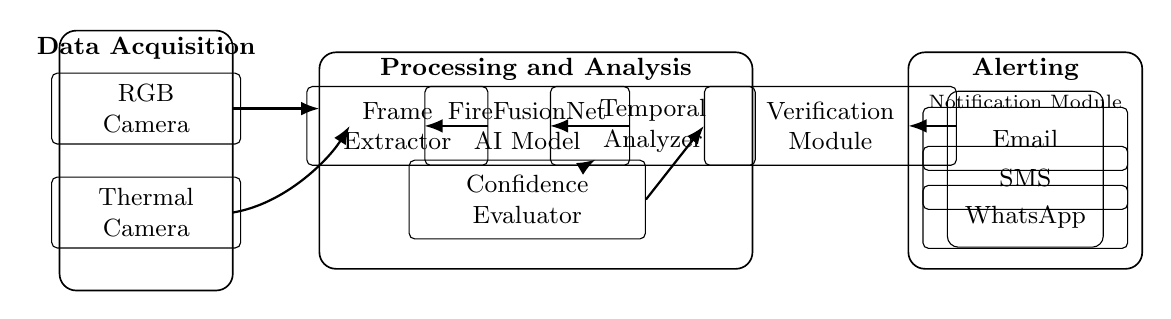
\begin{tikzpicture}[x=0.55cm,y=0.55cm,>=Latex,font=\small]
    % Data Acquisition box
    \draw[rounded corners=6pt, line width=0.6pt] (0,0) rectangle (4,6);
    \node at (2,5.6) {\bfseries Data Acquisition};
    \node[draw, rounded corners=2pt, minimum width=2.4cm, minimum height=0.9cm, align=center] (rgb) at (2,4.2) {RGB\\Camera};
    \node[draw, rounded corners=2pt, minimum width=2.4cm, minimum height=0.9cm, align=center] (thermal) at (2,1.8) {Thermal\\Camera};

    % Processing and Analysis box
    \draw[rounded corners=6pt, line width=0.6pt] (6,0.5) rectangle (16,5.5);
    \node at (11,5.1) {\bfseries Processing and Analysis};
    \node[draw, rounded corners=2pt, minimum width=2.3cm, minimum height=1.0cm, align=center] (frame) at (7.8,3.8) {Frame\\Extractor};
    \node[draw, rounded corners=2pt, minimum width=2.6cm, minimum height=1.0cm, align=center] (model) at (10.8,3.8) {FireFusionNet\\AI Model};
    \node[draw, rounded corners=2pt, minimum width=2.6cm, minimum height=1.0cm, align=center] (temporal) at (13.7,3.8) {Temporal\\Analyzer};
    \node[draw, rounded corners=2pt, minimum width=3.0cm, minimum height=1.0cm, align=center] (conf) at (10.8,2.1) {Confidence\\Evaluator};

    % Arrows from cameras to processing
    \draw[->, thick] (4,4.2) -- (6,4.2);
    \draw[->, thick] (4,1.8) .. controls (5.2,2.0) and (6.2,3.0) .. (6.7,3.8);

    % Chain arrows
    \draw[->, thick] (frame) -- (model);
    \draw[->, thick] (model) -- (temporal);
    \draw[->, thick] (temporal) -- (conf);

    % Verification module
    \node[draw, rounded corners=2pt, minimum width=3.2cm, minimum height=1.0cm, align=center] (verify) at (17.8,3.8) {Verification\\Module};
    \draw[->, thick] (conf.east) -- (verify.west);

    % Alerting box
    \draw[rounded corners=6pt, line width=0.6pt] (19.6,0.5) rectangle (25.0,5.5);
    \node at (22.3,5.1) {\bfseries Alerting};
    \draw[rounded corners=4pt] (20.5,1.0) rectangle (24.1,4.6);
    \node at (22.3,4.35) {\scriptsize Notification Module};
    \node[draw, rounded corners=2pt, minimum width=2.6cm, minimum height=0.8cm, align=center] at (22.3,3.5) {Email};
    \node[draw, rounded corners=2pt, minimum width=2.6cm, minimum height=0.8cm, align=center] at (22.3,2.6) {SMS};
    \node[draw, rounded corners=2pt, minimum width=2.6cm, minimum height=0.8cm, align=center] at (22.3,1.7) {WhatsApp};
    \draw[->, thick] (verify.east) -- (19.6,3.8);
  \end{tikzpicture}
  \caption{Drawn System Architecture (schematic).}
\end{figure}

\subsection{Data Strategy: Datasets and Augmentation}
Primary datasets include FASDD and D-Fire. Augmentations cover geometric transforms, photometric distortions, and advanced methods like Mosaic and MixUp.

\subsection{Model Architecture Details}
\begin{itemize}
  \item \textbf{Backbone (RGB--Thermal Fusion):} Dual streams with Efficient Attention Convolution (EAConv), merged via cross-modal attention gates.
  \item \textbf{Neck (Deformable Temporal Fusion):} Optical-flow-informed deformable convolutions with a lightweight temporal transformer to capture motion and reduce false alarms.
  \item \textbf{Head (Detection and Loss):} Multi-Scale Bi-Fusion Downsampling for small targets; composite Focal-SIoU-TriLoss combining regression, temporal consistency, and class-balanced terms.
\end{itemize}

\subsection{Training and Evaluation Plan}
We use cross-dataset curriculum pretraining, evaluate mAP, FPS, FPR/FNR, and benchmark against YOLOv8, YOLOGX, and DSS-YOLO on held-out test sets.

\subsection{Expected Contributions}
A robust multi-modal framework, an efficient real-time architecture for edge devices, strong cross-dataset generalization, and significant false-positive reduction via spatio-temporal reasoning.


% --------------- References ------------------
\section{References}
\begin{enumerate}
  \item\label{ismail2025survey} Ismail, N. D., Ramli, R., \& Ab Rahman, M. N. (2025). A systematic literature review of vision-based fire detection, prediction, and forecasting. \emph{Jurnal Kejuruteraan, 37}(1), 191--218. \url{https://doi.org/10.17576/jkukm-2025-37(1)-13}
  \item\label{sozol2025yolov5} Sozol, M. S. S., Mondal, M. R. H., \& Thamrin, A. H. (2025). Indoor fire and smoke detection based on optimized YOLOv5. \emph{PLOS ONE, 20}(4), e0322052. \url{https://doi.org/10.1371/journal.pone.0322052}
  \item\label{wang2025dssyolo} Wang, H., Fu, X., Yu, Z., \& Zeng, Z. (2025). DSS-YOLO: A lightweight real-time fire detection model based on an improved YOLOv8n. \emph{Scientific Reports, 15}, 8963. \url{https://doi.org/10.1038/s41598-025-93278-w}
  \item\label{mamadaliev2024esfd} Mamadaliev, D., Touko, P. L. M., Kim, J.-H., \& Kim, S.-C. (2024). ESFD-YOLOv8n: Early smoke and fire detection method based on an improved YOLOv8n model. \emph{Fire, 7}(9), 303. \url{https://doi.org/10.3390/fire7090303}
  \item\label{li2025yologx} Li, C., Du, Y., Zhang, X., \& Wu, P. (2025). YOLOGX: An improved forest fire detection algorithm based on YOLOv8. \emph{Frontiers in Environmental Science, 12}, 1486212. \url{https://doi.org/10.3389/fenvs.2024.1486212}
  \item\label{alkhammash2025compare} Alkhammash, E. H. (2025). A comparative analysis of YOLOv9, YOLOv10, YOLOv11 for smoke and fire detection. \emph{Fire, 8}(1), 26. \url{https://doi.org/10.3390/fire8010026}
  \item\label{ghali2022uav} Ghali, R., Akhloufi, M. A., \& Mseddi, W. S. (2022). Deep learning and transformer approaches for UAV-based wildfire detection and segmentation. \emph{Sensors, 22}(5), 1977. \url{https://doi.org/10.3390/s22051977}
  \item\label{xu2025genai} Xu, H., Zlatanova, S., Liang, R., \& Canbulat, I. (2025). Generative AI for predicting 2D and 3D wildfire spread: Beyond physics-based models and traditional deep learning. \emph{arXiv}. \url{https://doi.org/10.48550/arXiv.2506.02485}
  \item\label{kim2025vlm} Kim, J., Lee, Y., Yoon, D., Jung, C., \& Lee, G. (2025). An integrated YOLO and VLM system for fire detection in enclosed environments. ICLR 2025 Workshop. \url{https://openreview.net/forum?id=SKZuWQOHTh}
  \item\label{liu2025ffdnet} Liu, Q., Chen, H., \& Lin, D. (2025). Research and optimization of a multilevel fire detection framework based on deep learning and classical pattern recognition techniques. \emph{Scientific Reports, 15}, 20364. \url{https://doi.org/10.1038/s41598-025-06721-3}
  \item\label{kim2024multisensor} Kim, Y., Heo, Y., Jin, B., \& Bae, Y. (2024). Real-time fire classification models for an intelligent multi-sensor system. \emph{Fire, 7}(9), 329. \url{https://doi.org/10.3390/fire7090329}
  \item\label{zha2025lightfirenet} Zha, J.-H., Yang, Q.-Q., \& Lin, Y.-Q. (2025). LightFireNet: A lightweight forest fire recognition network based on knowledge distillation and FPGA acceleration. \emph{Forests, 16}(4), 698. \url{https://doi.org/10.3390/f16040698}
  \item\label{bu2025fireyolo} Bu, L., Li, W., Zhang, H., Wang, H., Tian, Q., \& Zhou, Y. (2025). FIRE-YOLOv8s: A lightweight and efficient algorithm for tunnel fire detection. \emph{Fire, 8}(4), 125. \url{https://doi.org/10.3390/fire8040125}
  \item\label{pan2024efa} Pan, W., Wang, X., \& Huan, W. (2024). EFA-YOLO: An efficient feature attention model for fire and flame detection. \emph{arXiv}. \url{https://arxiv.org/abs/2409.12635}
\end{enumerate}

\end{document}
